% based on Model 2 of Activity 12 - Recursion by Helen Hu, with modifications by Dee Weikle

\model{Summation}

''In mathematics, \emph{summation} (capital Greek sigma symbol: $\Sigma$) is the addition of a sequence of numbers; the result is their sum or total.''

$$ \sum_{i=1}^{100} i = 1 + 2 + 3 + \ldots + 100 = 5050 $$

\smallskip\hfill
Source: \url{https://en.wikipedia.org/wiki/Summation}


\quest{20 min}


\Q \label{sum4} Consider how to calculate $\sum\limits_{i=1}^{4} i = 10$.

\begin{enumerate}
\item Write out all the numbers that need to be added:

$\sum\limits_{i=1}^{4} i =$ \ans{4 + 3 + 2 + 1}

\item Showing how this sum can be calculated in terms of a smaller summation.

$\sum\limits_{i=1}^{4} i =$ \ans{4 + $\sum\limits_{i=1}^{3} i$}
\end{enumerate}


\Q \label{sumn} Write an expression similar to \ref{sum4}b showing how any summation of $n$ integers can be calculated in terms of a smaller summation.

\begin{center}
$\sum\limits_{i=1}^{n} i =$ \ans{n + $\sum\limits_{i=1}^{n-1} i$}
\end{center}


\Q What is the base case of the summation? (Write the complete formula, not just the value.)

\begin{answer}
$\sum\limits_{i=1}^{1} i = 1$
\end{answer}


\Q Implement a recursive method \java{summation} that takes a single parameter \java{n} and returns the sum $1 + 2 + \ldots + n$.
It should only have an \java{if} statement and two \java{return} statements.

\vspace{-1ex}
\begin{answer}[10em]
\begin{javaans}
public static int summation(int n) {
    if (n == 1) {
        return 1;
    } else {
        return n + summation(n - 1);
    }
}
\end{javaans}
\end{answer}


\Q Discuss how the \java{factorial} method below uses temporary variables.
What lines would you have to change to implement the \java{summation} method instead?

\begin{multicols}{2}

\vspace{1ex}
\begin{javalst}
public static int factorial(int n) {
    if (n == 0) {
        return 1;  // base case
    }
    int recurse = factorial(n - 1);
    int result = n * recurse;
    return result;
}
\end{javalst}

\columnbreak

\begin{answer}
The code is essentially the same, except that it would invoke \java{summation} instead of \java{factorial} and add terms instead of multiply.
You would also need to rename the method to \java{summation}.
\end{answer}

\end{multicols}


\Q Here is a stack diagram of ~\java{factorial(3)} when invoked from \java{main}.
Draw a similar diagram for \java{summation(3)} as described in the previous question.

\vspace{1em}
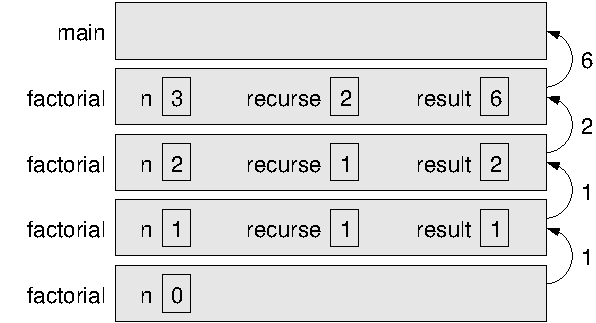
\includegraphics[width=0.5\linewidth]{stack-factorial3.pdf}
\vspace{1em}

%TODO solution for summation stack diagram


\Q Why are there no values for \java{recurse} and \java{result} in the stack diagram for the last call to \java{factorial} (when \java{n == 0})?

\begin{answer}
The method returns without declaring and using those variables.
\end{answer}


\Q Looking at the stack diagram, how is it possible that the parameter \java{n} can have multiple values in memory at the same time?

\begin{answer}
Each distinct method call has its own memory for parameters and local variables.
The value of \java{n - 1} in the first method call becomes the value of \java{n} in the next.
\end{answer}
